\section{The optimal setup}\label{sec:4:optimal-setup}
With the general framework in hand, the next logical question to ask is, if the stability against placement-variations can be improved.
The general rule of thumb for these optimizations is the following:
Increase the gravitational interaction by either heavier and larger particles or by reducing the separation distance $L$ without substantial sacrifices of experimental realization.
As an example, the stability increases intuitively by increasing the separation distance $L$. However, this does also increase the time $t_\mathrm{max}$ until the maximum amount of entanglement can be measured which would increase the total time  $\sim \# t_\mathrm{max}$ of the experiment with $\#$ individual measurements.
It is not immediately obvious, how the stability and the maximum possible variations $\Delta \theta_\mathrm{crit}$ and $\Delta L_\mathrm{crit}$ behave for the change in parameters.
In the following section, precisely the changing of this stability is discussed for changing the orientation $\alpha, \beta$, the separation $L$, the mass $M_A = M_B \equiv M$ and the superposition size $\Delta x_A = \Delta x_B \equiv \Delta x$.


\subsection{Orientation}
The arguably easiest parameter to change experimentally is the orientation of the superpositions, which is quantified by $\alpha$ and $\beta$ in \cref{fig:4:complete-setup}.
As already seen in \cref{fig:2:entanglement-dynamics}, the entanglement dynamics are dependent on the orientation.
In the parallel orientation, the states take twice as long as in the orthogonal orientation to become maximally entangled.
In general, it is advantageous to aim for the highest entanglement rate and thus the smallest $t_\mathrm{max}(\alpha, \beta)$, as this requires a shorter coherence time and thus reduces the total time of the experiment.
The previous results from \cref{cha:first-look} can be further generalized for an arbitrary orientation $\alpha, \beta$. The logarithmic negativity is given by
\begin{equation}
  E_N = \log_2\left(1+\abs{\sin\Delta\phi}\right)
\end{equation}
where $\Delta\phi$ is now dependent on the orientation and is defined as (for $\Delta x \ll L$)
\begin{equation}
  \Delta \phi = \frac{G M_A M_B t \Delta x_A \Delta x_B}{8\hbar L^3} \left(\sin\alpha\sin\beta-\frac{1}{2}\cos\alpha\cos\beta\right) .
\end{equation}
The maximum entanglement $E_N=1$ is reached for $\Delta\phi = \pm \pi/2$ and thus after a time
\begin{equation}\label{eq:4:t-max}
  t_\mathrm{max}(\alpha,\beta) = \frac{4\pi \hbar L^3}{G M_A M_B \Delta x_A \Delta x_B}\abs{\sin\alpha\sin\beta - \frac{1}{2}\cos\alpha\cos\beta}^{-1}.
\end{equation}
For some specific symmetric cases, the resulting times for different orientations are shown in \cref{fig:4:t-max-orientation}.
\begin{figure}[!htbp]
  \centering
  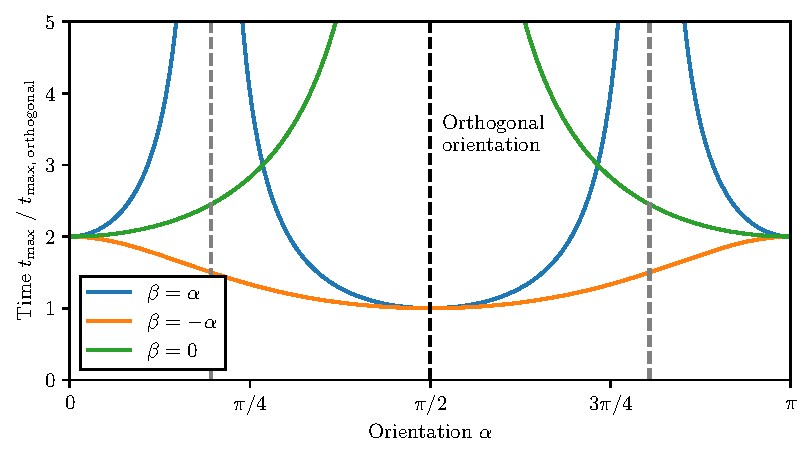
\includegraphics[width=\textwidth]{./../figures/ideal-entanglement/t-max-orientation.pdf}
  \caption{Time $t_\mathrm{max}$ after which maximum entanglement ($E_N = 1$) is reached for different orientations. Only the most interesting and highly symmetric cases $\alpha=\pm\beta$ and $\beta=0$ are shown. The singularity $t_\mathrm{max} \rightarrow \infty$ for $\beta = 0$ and $\alpha = \pi/2$ is expected. The two other singularities at $\alpha = \beta = 2 \arctan(\sqrt{3} \pm \sqrt{2})$ are explainable by the \q{harmonic mean} in \cref{fig:4:harmonic-mean}.}
  \label{fig:4:t-max-orientation}
\end{figure}
The global minima of $t_\mathrm{max}(\alpha,\beta)$ is attained in the orthogonal orientation. This is not surprising considering that this orientation maximizes the \textit{differences in separation distances} between all superposition states.
Much more interesting and surprising are the unanticipated singularities in \cref{fig:4:t-max-orientation} which appear for 
\begin{equation}
  \sin\alpha\sin\beta=\frac{1}{2}\cos\alpha\cos\beta .
\end{equation}
For $\beta=0$ the singularity at $\alpha=\pi/2$ is not surprising. In this configuration, the distances $\ket{\psi^1_A}\leftrightarrow\ket{\psi^{1,2}_B}$ and $\ket{\psi^2_A}\leftrightarrow\ket{\psi^{1,2}_B}$ are identical and thus these states accumulate the same phases, resulting in a factorable global phase.
In the case of $\alpha=\beta$, the two singularities are precisely given in the orientation
\begin{equation}
  \alpha=\beta=2 \arctan(\sqrt{3}\pm\sqrt{2})\approx 90\deg \pm 54.74\deg .
\end{equation}
There does not exist a straight-forward geometric interpretation why no entanglement is generated exactly in this configuration, however all 4 separation distances between the states form the \q{harmonic mean} visualized in \cref{fig:4:harmonic-mean}.
\begin{figure}[!htbp]
  \centering
  \def\svgwidth{\textwidth}
  \input{./../figures/harmonic-mean.pdf_tex}
  \caption{\textbf{left:} The system in the orientation $\alpha=\beta=2\arctan(\sqrt{3}-\sqrt{2})$. For $\Delta x \ll L$, all separation distances exactly form the \textit{harmonic mean}. Here, the phases due to the mutual gravitational interaction precisely cancel out resulting in no entanglement. \textbf{right:} Geometric visualization of the harmonic mean.}
  \label{fig:4:harmonic-mean}
  % COLORFUL:: $\textcolor[HTML]{aa0000}{\blacksquare} = \displaystyle\frac{2}{\frac{1}{\textcolor[HTML]{0044aa}{\blacksquare}}+\frac{1}{\textcolor[HTML]{447821}{\blacksquare}}}$
\end{figure}
Here, in the limit $\Delta x \ll L$ everything local phase precisely cancels out resulting in a loss of entanglement. 
To avoid all these singularities, it is advisable to always take $\alpha=-\beta$, where all orientations result in roughly similar entanglement times $t_\mathrm{max}$, at most only differing by a factor of $2$.

It should come as no surprise that the different orientations exhibit different stabilities. Logically, one would expect the orthogonal configuration to be much more sensitive to angular variations than the parallel one.
In contrary, the parallel configuration should be much more stable against variations in the distance, since no phase difference (\q{dephasing}) is induced between the two superposition states $\ket{\psi^1_{A(B)}}$ and $\ket{\psi^2_{A(B)}}$ of the particle $A$ ($B$).

The effect of different orientations on the stability against angular variations and the behavior of the critical angular variation $\Delta \theta_\mathrm{crit}$ is shown in \cref{fig:4:theta-crit-orientation}.
\begin{figure}[!htbp]
  \centering
  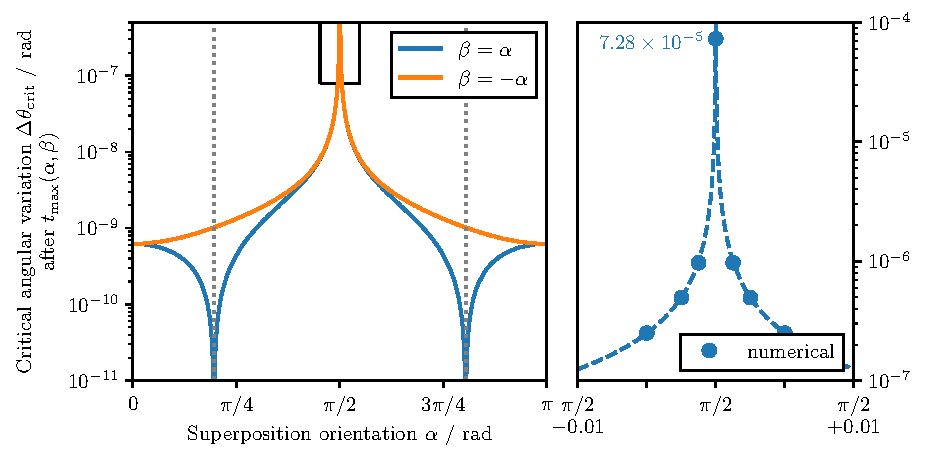
\includegraphics[width=\textwidth]{./../figures/theta-variance/theta-crit-orientation-complete.pdf}
  \caption{Critical angular variation $\Delta \theta_\mathrm{crit}$ for different orientations after the time $t_\mathrm{max}(\alpha, \beta)$ for which maximum entanglement is reached. The \emph{orthogonal orientation} magnified on the right is very stable against angular variations and only numerical methods show a finite stability value. The singularities in the left figure for $\alpha = \beta$ arise from the fact, that these orientations need infinite time to entangle as already seen in \cref{fig:4:t-max-orientation}.}
  \label{fig:4:theta-crit-orientation}
\end{figure}
As expected, the orthogonal configuration is the most stable against these kind of variations. This is, because the dephasing ultimately depends on the distance between the state and the shield $L \pm \Delta x/2 \cos\theta \approx L \pm \Delta x/2 (1 - \theta^2/2)$, which is a only second order effect of the angular variations $\theta$.
This explains the apparent \q{infinitely} good stability in the figure, as the analytical solution only uses first order approximations in $\theta$.
Exact numerical results however cap the stability at $\Delta \theta_\mathrm{crit,\,orthogonal} \approx 7.3\times 10^{-5}\si{rad}$.

Respectively, the stability against distance variations $\Delta L_\mathrm{crit}$ for different orientations is shown in \cref{fig:4:L-crit-orientation}.
\begin{figure}[!htbp]
  \centering
  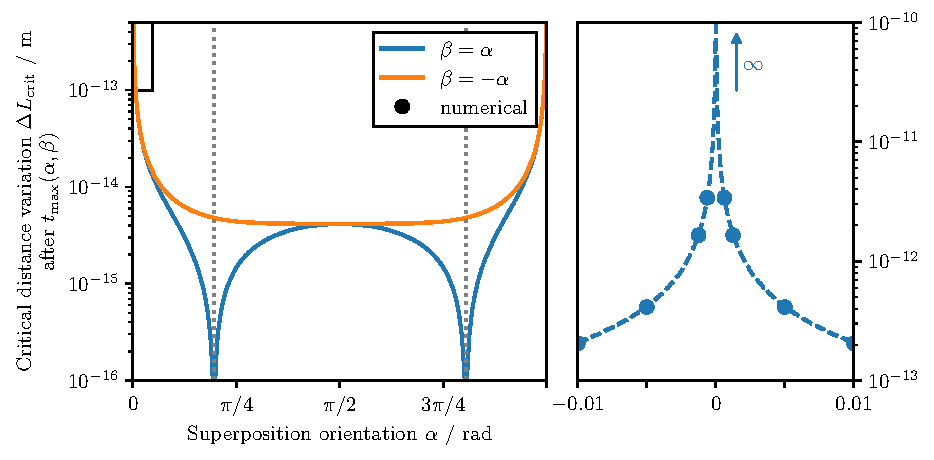
\includegraphics[width=\textwidth]{./../figures/L-variance/L-crit-orientation-complete.pdf}
  \caption{Critical distance variation $\Delta L_\mathrm{crit}$ for different orientations after a time $t_\mathrm{max}(\alpha,\beta)$. Here, the \emph{parallel orientation} (magnified on the left) is infinitely stable against placement variations.}
  \label{fig:4:L-crit-orientation}
\end{figure}
Again aligning with expectations, the parallel configuration is (in theory) exhibits an infinite stability.
One however could argue, that a for this to hold, the uncertainties in the angular placement have to be zero. As could be seen in \cref{fig:4:theta-crit-orientation}, these variations are at most around $\sim 5 \times 10^{-5}\si{rad}$ and thus a realistic upper bound for the minimum required distance variations is given by $\Delta L_\mathrm{crit,parallel} = \Delta L_\mathrm{crit}(\alpha \approx 5\times 10^{-5}\si{rad}) \simeq 4\times 10^{-11}\si{m}$.
It is important to keep in mind, that these stability values can be improved substantially by changing e.g. the separation distance $L$ or the particle size $R$.

Considering these results, the parallel orientation seems to be the only realistic experimental option, even if it requires slightly larger coherence times $t_\mathrm{max}$.
Keeping particle-shield separation variations below $0.01\si{nm}$ - approximately the size of a single atom - is practically impossible,  
especially under the additional consideration of the thermal vibrations of the shield and the particles, which are in the same order of magnitude as seen later in \cref{cha:the-shield}.
With this data on hand, it is possible to generate the stability diagram in \cref{fig:4:optimal-orientation}, showing the optimal orientation in which the most entanglement can be measured.
For most combinations of $\Delta L$ and $\Delta \theta$, entanglement is only given in one certain orientation.
\begin{figure}[!htbp]
  \centering
  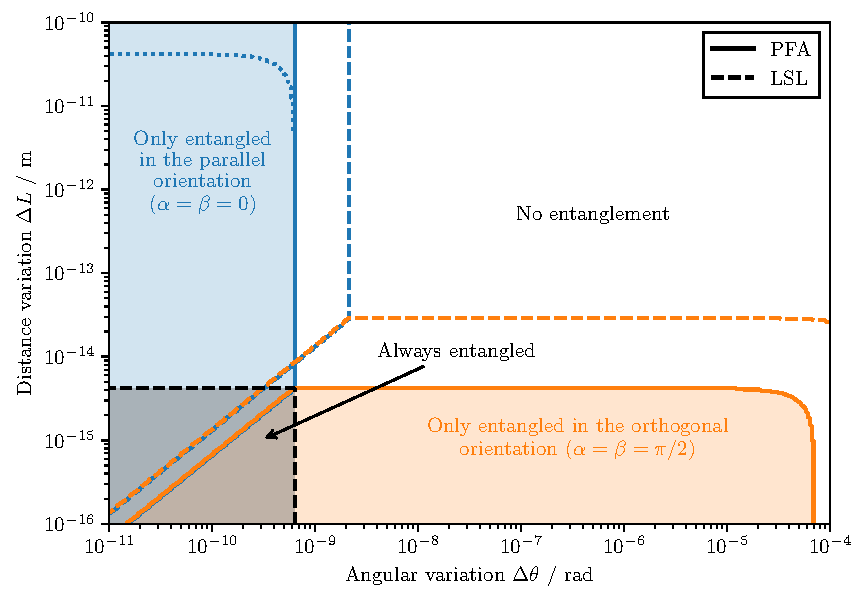
\includegraphics[width=\textwidth]{./../figures/optimize/optimized-orientation-advanced.pdf}
  \caption{Optimal orientation for the experimental setup dependent on the variations in angle $\Delta\theta$ and distance $\Delta L$ for a initial separation distance of $L=2R=2\times 10^{-5}\si{m}$ at time $t_\mathrm{max}$. The different predictions for the proximity-force-approximation (PFA) and the large-separation-limit (LSL) are shown. At a distance of $L=20\si{\mu m}$ the actual casimir interaction is somewhere in the middle between both approximations. In the region where entanglement is given regardless of the orientation (the bottom left), the orientation with \textit{more} entanglement is still colored. The dotted line corresponds to the realistic upper bound discussed in the text.}
  \label{fig:4:optimal-orientation}
\end{figure}


\newpage
\subsection{Separation, mass and superposition size}
It is possible to improve the required stability in placement and consequently the entanglement generation by changing the other parameters shown in \cref{fig:4:complete-setup} besides the orientation. 
It is especially easy to modify the separation distance $L$ during the experiment as one is only limited in the trap stability close to the shield discussed in \cref{sec:4:trapping}. The other parameters like the particle mass $M$ and thus the radius $R$, the particle material and the superposition size $\Delta x$ are considerably more difficult to change.  
One is limited by the experimental implementation of the spatial superpositions. Considering that up to date, the largest spatial superposition of a \q{macroscopic object} is in the order of $\Delta x \sim 500\si{nm}$ for masses of $4\times 10^{-23}\si{kg}$ \cite{Fein_2019}, large changes in the delocalization size $\Delta x$ or the particles mass might be virtually impossible.
However, out of a theoretical standpoint, the effects of all these parameters and the improvements reachable in stability are interesting and considered in the following section.

Beginning with the effect of a larger particle-shield separation $L$, the improvements on angular stability are shown in \cref{fig:4:theta-crit-L}.
\begin{figure}[!htbp]
  \centering
  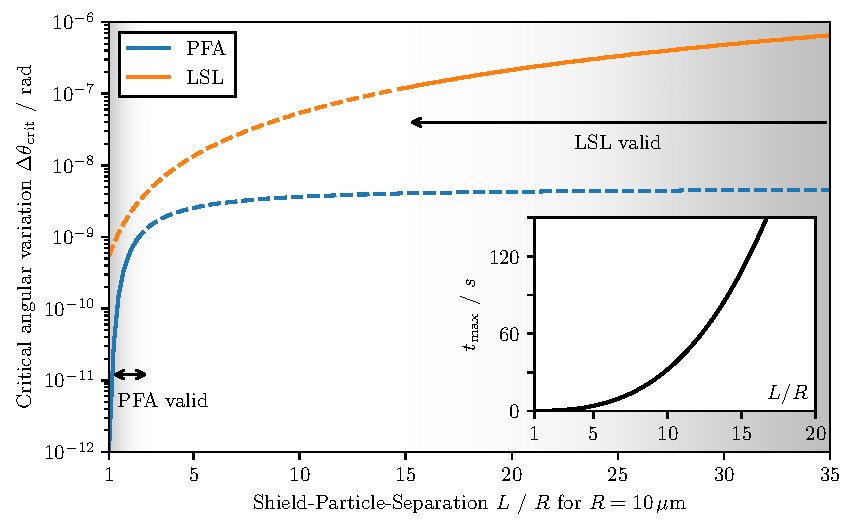
\includegraphics[width=\textwidth]{./../figures/theta-variance/theta-crit-L.pdf}
  \caption{Stability against angular variations for increasing separation distances $L$ in units of $R=10\si{\mu m}$ after a time $t_\mathrm{max}(L)$. The dependence on the radius can be seen in \cref{fig:4:theta-crit-mass}. Two models for the casimir-interaction are shown: The proximity-force-approximation (PFA) and the large-separation-limit (LSL). The regions outside the models validity are indicated with dashed lines. In the bottom right the time $t_\mathrm{max}(L) \propto L^3$ is shown.}
  \label{fig:4:theta-crit-L}
\end{figure}
A similar figure can be created for the stability of distance-variations $\Delta L$, but as already discussed previously, the setup is very (infinitely) stable against small distance variations in the parallel configuration.
It is intuitively clear that a larger separation improves the stability, as the relative effect of the variations $\sim \Delta x \sin\theta \ll L$ decreases and the Casimir potential tends towards zero.
However, a larger separation also increases the time $t_\mathrm{max} \propto L^3$ until the maximum entanglement is built up.
The combination of both effects leads to the result shown in \cref{fig:4:theta-crit-L}.
Due to the strong distance dependence on the casimir model, both limits for either small separations $L \sim R$ (PFA) or large separations $L \gg R$ (LSL) have been compared. 
The \q{real} casimir potential lies somewhere between the two models.
In general, it can be said, that a large separation is desirable, as long as the required coherence times are still reachable.

The mass of the particles is determined by their radius $R$ as well as their material.
Most likely, the trapped and levitated particles are made of silica ($\mathrm{SiO_2}$) with a density of $\rho_\mathrm{Silica} = 2648\si{kg/m^3}$, as this material has been used widely in experiments on levitated nanoparticles \cite{Grass_2016,Slezak_2018}. Due to its transparency, silica is very easy to trap in strong optical traps, but even quantum control in magnetic traps has been demonstrated with silica \cite{Slezak_2018}.
For this thesis, I will assume that all trapped particles are made of silica. Otherwise denser or heavier materials like e.g. stable osmium and lead isotopes would be worth considering.
Trapping them in a paramagnetic trap could be theoretically possible and interesting as sufficient masses could already be reached with far fewer atoms and smaller particles, further improving coherence times and quantum control.
The effect on angular stability of a larger and thus heavier particle is shown in \cref{fig:4:theta-crit-mass}.
\begin{figure}[!htbp]
  \centering
  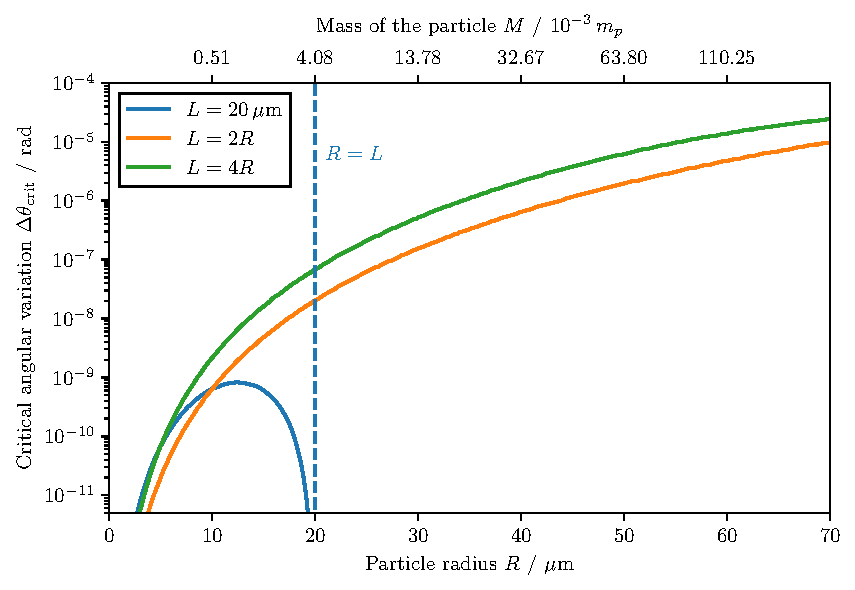
\includegraphics[width=\textwidth]{./../figures/theta-variance/theta-crit-mass.pdf}
  \caption{Critical angular variation $\Delta \theta_\mathrm{crit}$ for different sized particles after a time $t_\mathrm{max}(M)$. The mass of the corresponding particle in units of the Planck mass $m_p = \sqrt{\hbar c / G} \approx 2.176\times 10^{-8}\si{kg}$ is given on the top axis. For particles as large as the separation $R = L$, the surface-to-surface separation is almost zero, resulting in large casimir forces and thus no entanglement.}
  \label{fig:4:theta-crit-mass}
\end{figure}
It is important to note, that the time $t_\mathrm{max}$ scales with $M^{-2}$ and thus effectively with $R^{-6}$, making the effect of a slightly larger sphere very noticeable.
One does need to find the ideal size of the sphere depending on what is possible experimentally: The mass must be large enough for gravity to have a measurable effect but simultaneously small enough for sufficient quantum control in the laboratory. 
Estimations suggest the usage of masses around the order of $10^{-11}\si{kg} \approx 10^{-3}\,m_p$ as being possible \cite{Aspelmeyer_2024}.

The final parameter that theoretically be freely modified, is the size of the superposition $\Delta x$. A larger superposition size would increase the entanglement generation due to gravity because the differences in the distances between all superposition states would increase. Such effects ultimately lead to a faster build-up of entanglement scaling with $t_\mathrm{max} \propto (\Delta x)^{-2}$.
In matter wave experiments, superposition sizes of massive objects up to $\Delta x \approx 500\si{nm}$ were already achieved \cite{Fein_2019}.
These sizes are much smaller than the size of the particle itself at $10\si{\mu m}$.
The effect of the superposition size on stability is shown in \cref{fig:4:theta-crit-superposition-size}.
\begin{figure}[!htbp]
  \centering
  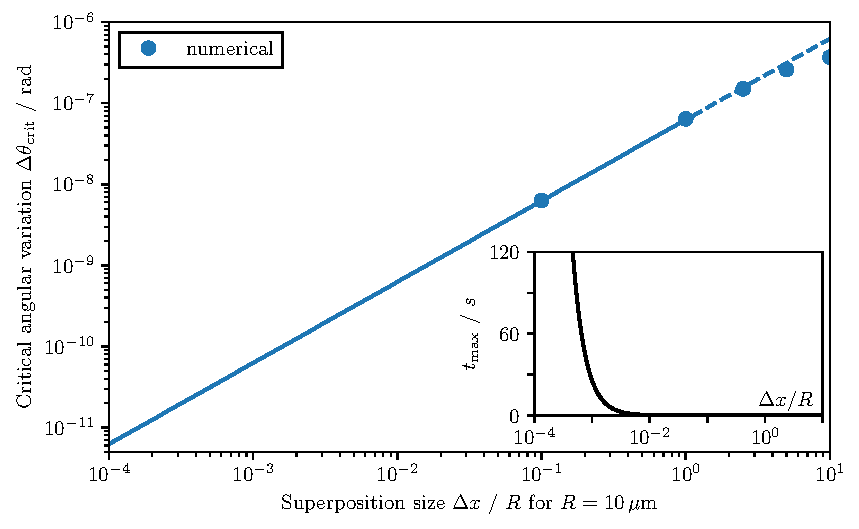
\includegraphics[width=\textwidth]{./../figures/theta-variance/theta-crit-superpos-size.pdf}
  \caption{Effect of the superposition size $\Delta x$ on the critical angular stability $\Delta \theta_\mathrm{crit}$ after a time $t_\mathrm{max}(\Delta x)$. For $\Delta x \gtrsim R$, numerical results are used. In the lower left, the time till maximum entanglement $t_\mathrm{max} \propto (\Delta x)^{-2}$ is shown. For $\Delta x \ll R$, the resulting relation between $\Delta x$ and $\Delta \theta_\mathrm{crit}$ is linear.}
  \label{fig:4:theta-crit-superposition-size}
\end{figure}
For large superposition sizes, the time until maximal entanglement is reached, decreases drastically. In the shorter time, the dephasing due to the casimir effect between the shield and the states is less substantial, increasing the stability against variations in the placement.
A larger superposition size on the other hand results in a greater effect of angular variations $\sim \Delta x \sin(\theta)$.
Both of these effects result in a effective scaling of $\sim \Delta x$, which explains the linear curve\footnote{Here it is shown in a double-logarithmic plot. The relation between $\Delta x$ and $\Delta \theta_\mathrm{crit}$ is nevertheless linear. Proofing the linearity is not straightforward. The following argument can be made: $E_N = \log_2(1 + f(x)) \approx f(x)/\log(2)$ where $f(x)$ is related to the decoherences and the off-diagonal elements of the state $\mean{\rho}$. Thus, it is dependent on $t$ and to the angular variations $\sim \Delta x$ (see \cref{apx:average-density}) resulting in a decoherence of $\sim t \Delta x \propto 1/(\Delta x)$ and thus in a linear improvement for larger superposition sizes.}.



